\documentclass[tikz, border=0]{standalone}
\usepackage{tikz}
\begin{document}
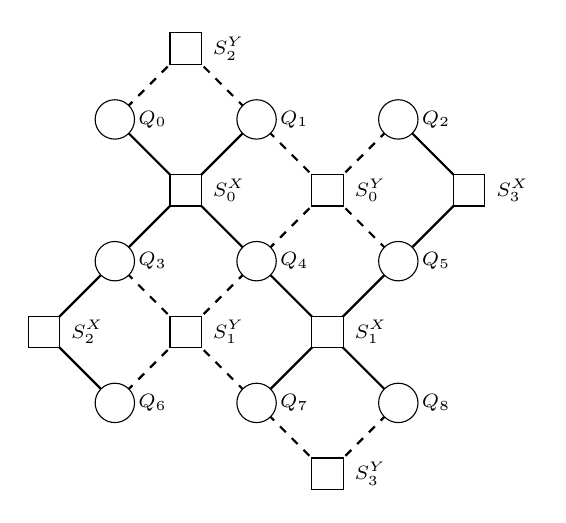
\begin{tikzpicture}
\draw[black,thick,solid] (0.0,3.6) -- (0.9,2.7);
\draw[black,thick,solid] (1.8,3.6) -- (0.9,2.7);
\draw[black,thick,solid] (0.0,1.8) -- (0.9,2.7);
\draw[black,thick,solid] (1.8,1.8) -- (0.9,2.7);
\draw[black,thick,solid] (1.8,1.8) -- (2.7,0.9);
\draw[black,thick,solid] (3.6,1.8) -- (2.7,0.9);
\draw[black,thick,solid] (1.8,0.0) -- (2.7,0.9);
\draw[black,thick,solid] (3.6,0.0) -- (2.7,0.9);
\draw[black,thick,solid] (0.0,1.8) -- (-0.9,0.9);
\draw[black,thick,solid] (0.0,0.0) -- (-0.9,0.9);
\draw[black,thick,solid] (3.6,3.6) -- (4.5,2.7);
\draw[black,thick,solid] (3.6,1.8) -- (4.5,2.7);
\draw[black,thick,dashed] (1.8,3.6) -- (2.7,2.7);
\draw[black,thick,dashed] (3.6,3.6) -- (2.7,2.7);
\draw[black,thick,dashed] (1.8,1.8) -- (2.7,2.7);
\draw[black,thick,dashed] (3.6,1.8) -- (2.7,2.7);
\draw[black,thick,dashed] (0.0,1.8) -- (0.9,0.9);
\draw[black,thick,dashed] (1.8,1.8) -- (0.9,0.9);
\draw[black,thick,dashed] (0.0,0.0) -- (0.9,0.9);
\draw[black,thick,dashed] (1.8,0.0) -- (0.9,0.9);
\draw[black,thick,dashed] (0.0,3.6) -- (0.9,4.5);
\draw[black,thick,dashed] (1.8,3.6) -- (0.9,4.5);
\draw[black,thick,dashed] (1.8,0.0) -- (2.7,-0.9);
\draw[black,thick,dashed] (3.6,0.0) -- (2.7,-0.9);
\filldraw[fill=white, draw=black] (0.0,3.6) circle (0.25) node at (0.175,3.6) [right] {$\scriptstyle Q_{0}$};
\filldraw[fill=white, draw=black] (1.8,3.6) circle (0.25) node at (1.975,3.6) [right] {$\scriptstyle Q_{1}$};
\filldraw[fill=white, draw=black] (3.6,3.6) circle (0.25) node at (3.775,3.6) [right] {$\scriptstyle Q_{2}$};
\filldraw[fill=white, draw=black] (0.0,1.8) circle (0.25) node at (0.175,1.8) [right] {$\scriptstyle Q_{3}$};
\filldraw[fill=white, draw=black] (1.8,1.8) circle (0.25) node at (1.975,1.8) [right] {$\scriptstyle Q_{4}$};
\filldraw[fill=white, draw=black] (3.6,1.8) circle (0.25) node at (3.775,1.8) [right] {$\scriptstyle Q_{5}$};
\filldraw[fill=white, draw=black] (0.0,0.0) circle (0.25) node at (0.175,0.0) [right] {$\scriptstyle Q_{6}$};
\filldraw[fill=white, draw=black] (1.8,0.0) circle (0.25) node at (1.975,0.0) [right] {$\scriptstyle Q_{7}$};
\filldraw[fill=white, draw=black] (3.6,0.0) circle (0.25) node at (3.775,0.0) [right] {$\scriptstyle Q_{8}$};
\filldraw[fill=white, draw=black] (0.7,2.5) rectangle (1.1,2.9000000000000004) node at (1.12,2.7) [right] {$\scriptstyle S^X_{0}$};
\filldraw[fill=white, draw=black] (2.5,0.7) rectangle (2.9000000000000004,1.1) node at (2.9200000000000004,0.9) [right] {$\scriptstyle S^X_{1}$};
\filldraw[fill=white, draw=black] (-1.1,0.7) rectangle (-0.7,1.1) node at (-0.6799999999999999,0.9) [right] {$\scriptstyle S^X_{2}$};
\filldraw[fill=white, draw=black] (4.3,2.5) rectangle (4.7,2.9000000000000004) node at (4.72,2.7) [right] {$\scriptstyle S^X_{3}$};
\filldraw[fill=white, draw=black] (2.5,2.5) rectangle (2.9000000000000004,2.9000000000000004) node at (2.9200000000000004,2.7) [right] {$\scriptstyle S^Y_{0}$};
\filldraw[fill=white, draw=black] (0.7,0.7) rectangle (1.1,1.1) node at (1.12,0.9) [right] {$\scriptstyle S^Y_{1}$};
\filldraw[fill=white, draw=black] (0.7,4.3) rectangle (1.1,4.7) node at (1.12,4.5) [right] {$\scriptstyle S^Y_{2}$};
\filldraw[fill=white, draw=black] (2.5,-1.1) rectangle (2.9000000000000004,-0.7) node at (2.9200000000000004,-0.9) [right] {$\scriptstyle S^Y_{3}$};
\end{tikzpicture}
\end{document}
